\documentclass[final,12pt]{colt2018} % Anonymized submission
% \documentclass{colt2017} % Include author names
% !TeX root = main.tex

%%% USED FOR COMMENTS

\def\a{\alpha}
\def\b{\beta}
\def\c{\chi}
\def\d{\delta}
\def\D{\Delta}
%\def\e{\epsilon}
\def\e{\eta}
\def\eps{\ve}
\renewcommand{\epsilon}{\ve}
\def\ve{\varepsilon}
\def\f{\phi}
\def\F{\Phi}
\def\g{\gamma}
\def\G{\Gamma}
\def\k{\kappa}
\def\K{\Kappa}
\def\z{\zeta}
\def\th{\theta}
\def\Th{\Theta}
\def\l{\lambda}
\def\la{\lambda}
%\def\L{\Lambda}
\def\m{\mu}
\def\n{\nu}
\def\p{\pi}
\def\P{\Pi}
\def\r{\rho}
\def\R{\Rho}
\def\s{\sigma}
\def\S{\Sigma}
\def\t{\tau}
\def\om{\omega}
\def\Om{\Omega}
\def\smallo{{\rm o}}
\def\bigo{{\rm O}}
\def\to{\rightarrow}
\def\ex{{\bf Exp}}
\def\cd{{\cal D}}
\def\rme{{\rm e}}
\def\hf{{1\over2}}
\def\R{{\bf  R}} 
\def\cala{{\cal A}}
\def\calt{{\cal T}}
\def\cale{{\cal E}}
\def\Fscr{{\cal F}}
\def\cc{{\cal C}}
\def\calc{{\cal C}}
\def\call{{\cal L}}
\def\calm{{\cal M}}
\def\calh{{\cal H}}
\def\cali{{\cal I}}
\def\bk{\backslash}


\newcommand{\Exp}{\E}
\newcommand{\E}{\mbox{\bf E}}
\newcommand{\Var}{\mbox{\bf Var}}
\newcommand{\sign}{\mbox{\bf sign}}

\newcommand{\erf}{\mbox{\text erf}}
\newcommand{\erfc}{\mbox{\text erfc}}

\newcommand{\pr}[2][]{\mbox{Pr}\ifthenelse{\not\equal{}{#1}}{_{#1}}{}\!\left[#2\right]}
\newcommand{\given}{\ \mid\ }
\newcommand{\reals}{\mathbb{R}}

\newcommand{\U}{\mathcal{U}_n}


\newcommand{\limninf}{\lim_{n \rightarrow \infty}}
\newcommand{\proofstart}{{\bf Proof\hspace{2em}}}
\newcommand{\tset}{\mbox{$\cal T$}}
\newcommand{\proofend}{\hspace*{\fill}\mbox{$\Box$}}
\newcommand{\bfm}[1]{\mbox{\boldmath $#1$}}
%\newcommand{\reals}{\mbox{\bfm{R}}}
%\newcommand{\expect}{\mbox{\bf Exp}}
\newcommand{\he}{\hat{\e}}
\newcommand{\card}[1]{\mbox{$|#1|$}}
\newcommand{\rup}[1]{\mbox{$\lceil{ #1}\rceil$}}
\newcommand{\rdn}[1]{\mbox{$\lfloor{ #1}\rfloor$}}
\newcommand{\ov}[1]{\mbox{$\overline{ #1}$}}
\newcommand{\inv}[1]{$\frac{1}{ #1}$}
\newcommand{\dtv}{d_{\mathrm {TV}}}
\newcommand{\dk}{d_{\mathrm K}}
\newcommand{\dkl}{d_{\mathrm {KL}}}
\newcommand{\dskl}{d_{\mathrm {SKL}}}
\newcommand{\Tr}{{\mathrm {Tr}}}


\newcommand{\ignore}[1]{}
\providecommand{\poly}{\operatorname*{poly}}

\newenvironment{proofsketch}{\noindent {\em {Proof (sketch):}}}{$\blacksquare$\vskip \belowdisplayskip}
\newenvironment{prevproof}[2]{\noindent {\em {Proof of {#1}~\ref{#2}:}}}{$\hfill\qed$\vskip \belowdisplayskip}

%\newenvironment{prevproof}[2]{\noindent {\em {Proof of
%{#1}~\ref{#2}:}}}{$\blacksquare$\vskip \belowdisplayskip}

% Allow argmax operation
\DeclareMathOperator{\lcm}{lcm}
\DeclareMathOperator{\img}{img}
\DeclareMathOperator{\GL}{GL}
\DeclareMathOperator{\argmax}{argmax}
\DeclareMathOperator{\avg}{avg}

%\def\qedsymbol{\blksquare}
\newcommand{\bg}[1]{\medskip\noindent{\bf #1}}
%\newcommand{\ed}{{\hfill\qedsymbol}\medskip}
\newenvironment{proofof}[1]{\bg{Proof of #1 : }}{\qed}



%%%
%%% Packed enumerate / itemize
%%%

\newenvironment{packed_enum}{
\begin{enumerate}
  \setlength{\itemsep}{0pt}
  \setlength{\parskip}{0pt}
  \setlength{\parsep}{0pt}
}{\end{enumerate}}

\newenvironment{packed_item}{
\begin{itemize}
  \setlength{\itemsep}{0pt}
  \setlength{\parskip}{0pt}
  \setlength{\parsep}{0pt}
}{\end{itemize}}

\definecolor{Red}{rgb}{1,0,0}
\def\red{\color{Red}}
\newcommand{\costasnote}[1]{{\red #1}}
\newcommand{\oldbound}[1]{{}}


\newcommand{\sparse}{\mathrm{sparse}}
\newcommand{\lrg}{\mathrm{large}}

\newcommand{\Loss}{\text{Loss}}
\newcommand{\Unif}{\text{Uniform}}
\newcommand{\Ind}{\mathbb{I}}
\newcommand{\Supp}{\text{supp}}
\newcommand{\Inv}{\textsc{Inv}}

% The following packages will be automatically loaded:
% amsmath, amssymb, natbib, graphicx, url, algorithm2e

\title[Actively Avoiding Nonsense in Generative Models]{Actively Avoiding Nonsense in Generative Models}
\usepackage{times}
\usepackage{algorithmic}
 % Use \Name{Author Name} to specify the name.
 % If the surname contains spaces, enclose the surname
 % in braces, e.g. \Name{John {Smith Jones}} similarly
 % if the name has a "von" part, e.g \Name{Jane {de Winter}}.
 % If the first letter in the forenames is a diacritic
 % enclose the diacritic in braces, e.g. \Name{{\'E}louise Smith}

 % Two authors with the same address
  % \coltauthor{\Name{Author Name1} \Email{abc@sample.com}\and
  %  \Name{Author Name2} \Email{xyz@sample.com}\\
  %  \addr Address}

 % Three or more authors with the same address:
 % \coltauthor{\Name{Author Name1} \Email{an1@sample.com}\\
 %  \Name{Author Name2} \Email{an2@sample.com}\\
 %  \Name{Author Name3} \Email{an3@sample.com}\\
 %  \addr Address}


 % Authors with different addresses:
 \coltauthor{\Name{Steve Hanneke} \Email{steve.hanneke@gmail.com}\\
 \addr Princeton, NJ
 \AND
 \Name{Adam Tauman Kalai} \Email{adum@microsoft.com}\\%I'm happy to be last author if you choose not to go alphabetically.
 \addr Microsoft Research, New England
 \AND
 \Name{Gautam Kamath} \Email{g@csail.mit.edu}\\
 \addr EECS \& CSAIL, MIT
 \AND
 \Name{Christos Tzamos} \Email{chtzamos@microsoft.com}\\
 \addr Microsoft Research, New England
 }

\begin{document}

\maketitle

\begin{abstract}
A generative model may generate utter nonsense when it is fit to maximize the likelihood of observed data. This happens due to ``model error,'' i.e., when the true data generating distribution does not fit within the class of generative models being learned. To address this, we propose a model of active distribution learning using a binary invalidity oracle that identifies some examples as clearly invalid, together with random positive examples sampled from the true distribution. The goal is to maximize the likelihood of the positive examples subject to the constraint of (almost) never generating examples labeled invalid by the oracle. Guarantees are agnostic compared to a class of probability distributions. We first show that proper learning may require exponentially many queries to the invalidity oracle. We then give an improper distribution learning algorithm that uses only polynomially many queries. 
%Our algorithm is a polynomial-time reduction to a supervised generative modeling problem.
\end{abstract}

\begin{keywords}
Generative models, active learning, statistical learning
\end{keywords}

% !TeX root = main.tex
\section{Introduction}
\label{sec:intro}
Generative models are often trained in an unsupervised fashion, fitting a model $q$ to a set of observed data $x_P \subseteq X$ drawn iid from some true distribution $p$ on $x\in X$. Now, of course $p$ may not exactly belong to family $Q$ of probability distributions being fit, whether $Q$ consists of Gaussians mixture models, Markov models, or even neural networks of bounded size. We first discuss the limitations of generative modeling without feedback, and then discuss our model and results.

%\subsection{Limitations of Generative Modeling from Positive Examples Alone}
Consider fitting a generative model on a text corpus consisting partly of poetry written by four-year-olds and partly of mathematical publications from the {\em Annals of Mathematics}. Suppose that learning to generate a poem that looks like it was written by a child was easier than learning to generate a novel mathematical article with a correct, nontrivial statement. If the generative model pays a high price for generating unrealistic examples, then it may be better off learning to generate children's poetry than mathematical publications. However, without negative feedback, it may be difficult for a neural network or any other model to know that the mathematical articles it is generating are stylistically similar to the mathematical publications but do not contain valid proofs.\footnote{This is excluding clearly fake articles published without proper review in lower-tier venues \citep{LabbeL13}.} 

As a simpler example, the classic Markovian ``trigram model'' of natural language assigns each word a fixed probability conditioned only on the previous two words. Prior to recent advances in deep learning, for decades the trigram model and its variant were the workhorses of language modeling, assigning much greater likelihood to natural language corpora than numerous linguistically motivated grammars and other attempts \citep{Rosenfeld00}. However, text sampled from a trigram is typically nonsensical, e.g., the following text was randomly generated from a trigram model fit on a corpus of text from the Wall Street Journal \citep{JurafskyM09}:
\begin{quote}
They also point to ninety nine point six billion dollars from two hundred
four oh six three percent of the rates of interest stores as Mexico and
gram Brazil on market conditions. 
\end{quote}

In some applications, like text compression using a language model \citep{WittenNC87}, maximizing likelihood is equivalent to optimizing compression. However, in many  applications involving generation, such nonsense is costly and unacceptable. Now, of course it is possible to always generate valid data by returning random training examples, but this is simply overfitting and not learning. Alternatively, one could incorporate human-in-the-loop feedback such as through crowdsourcing, into the generative model to determine what is a valid, plausible sentence.

In some domains, validity could be determined automatically. Consider a Markovian model of a well-defined concept such as mathematical formulas that compile in \LaTeX{}. Now, consider a $n$-gram Markovian character model which the probability of each subsequent character is determined by the previous $n$ characters. For instance, the expression \$\{2+\{x-y\}\$ is invalid in \LaTeX{} due to mismatched braces. For this problem, a \LaTeX{} compiler may serve as a validity oracle. Various $n$-gram models can be fit which only generate valid formulas. To address mismatched braces, for example, one such model would ensure that it always closed braces within $n$ characters of opening, and had no nested braces. While an $n$-gram model will not perfectly model the true distribution over valid \LaTeX{} formulas, for certain generative purposes one may prefer an $n$-gram model that generates valid formulas over one that assigns greater likelihood to the training data but generates invalid formulas. 

Figure \ref{fig:rectangle} illustrates a simple case of learning a rectangle model for data which is not uniform over a rectangle. A maximum likelihood model would necessarily be the smallest rectangle containing all the data, but most examples generated from this distribution may be invalid. Instead a smaller rectangle, as illustrated in the figure, may be desired.

\begin{figure}[h]\label{fig:rectangle}
\centering
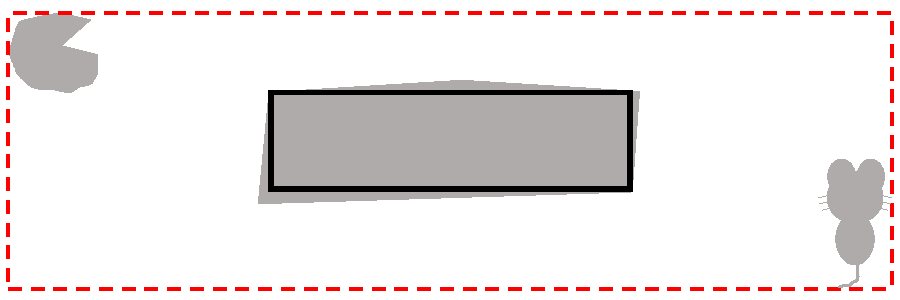
\includegraphics[width=3in]{fig.pdf}
\caption{Example where the underlying distribution $p$ is uniform over the (gray) valid regions. The solid rectangle maximizes our objective since it does not output nonsense (is supported only within the grey matter) and is closest to the $p$ (covers the maximum amount of grey matter). In contrast, the standard maximum likelihood (dashed red) rectangle must fully contain the observed samples, thus generating invalid points most of the time.  }
\end{figure}

Motivated by these observations, we evaluate a generative model $q$ on two axes. First is {\em coverage}, which is related to the probability assigned to future examples drawn from the true distribution $p$. Second is {\em validity}, defined as the probability that random examples generated from $q$ meet some validity requirement. Formally, we measure coverage in terms of a bounded {\em loss}:
$$\Loss(p,q)=\E_{x \sim p}[L(q_x)],$$
where $L:[0,1]\rightarrow [0,M]$ is a bounded decreasing function such as the capped log-loss $L(q_x)=\min(M, \log 1/q_x)$. % or $L(q_x)=\log 1/(q_x+\exp(-M))$. 
A bounded loss has the advantages of being efficiently estimable, and also it enables a model to assign 0 probability to one example (e.g., an outlier or error) if it greatly increases the likelihood of all other data. Validity is defined with respect to a set $V \subseteq X$, and $q(V)$ is the probability that a random example generated from $q$ lies within $V$. 

Clearly, there is a tradeoff between coverage and validity. We first focus on the case of (near) perfect validity. A Valid Generative Modeling (VGM) algorithm if it outputs, for a family of distributions $Q$ over $X$, if it outputs $\hat{q}$ with (nearly) perfect validity and whose loss is nearly as good as the loss of the best valid $q\in Q$. More precisely, $A$ is a VGM learner of $Q$ if for any nonempty valid subset $V \subseteq X$, any probability distribution $p$ over $V$, and any $\eps>0$, $A$ uses $n$ random samples from $p$ and makes $m$ membership oracle calls to $V$ and outputs a distribution $\hat{q}$ such that, $$\Loss(p, \hat{q}) \leq \min_{q \in Q: q(V)=1}\Loss(p,q) + \eps ~\text{ and }~\hat{q}(V)\geq 1-\eps.$$ 
We aim for our learner to be sample and query efficient, requiring that $n$ and $m$ are polynomial in $M, 1/\eps$ and a measure of complexity of our distribution class $Q$.
Furthermore, we would like our algorithms to be computationally efficient, with a runtime polynomial in the size of the data, namely the $n + m$ training examples. 
A more formal description of the problem is available in Section~\ref{sec:problem}.

$A$ is said to be {\em proper} if it always outputs $\hat{q}\in Q$ and {\em improper} otherwise.
In Section~\ref{sec:impossibility}, we first show that efficient proper learning for VGM is impossible. This is an information-theoretic result, meaning that even given infinite runtime and positive samples, one still cannot solve the VGM problem. Interestingly, this is different from binary classification, where it is possible to statistically learn from iid examples without a membership oracle.

Our first main positive result is an efficient (improper) learner for VGM. The algorithm relies on a subroutine that solves the following {\em Generative Modeling with Negatives} (GMN) problem: given sets $X_P, X_N \subset X$ of positive and negative examples, find the probability distribution $q \in Q$ which minimizes $\sum_{x \in X_P} L(q(x))$ subject to the constraint that $q(X_N)=0$. For simplicity, we present our algorithm for the case that the distribution family $Q$ is finite, giving sample and query complexity bounds that are logarithmic in terms of $|Q|$. However, as we show in Section~\ref{sec:infinite-families}, all of our results extend to infinite families $Q$. It follows that if one has a computationally efficient algorithm for the GMN problem for a distribution family $Q$, then our reduction gives a computationally efficient VGM learning algorithm for $Q$.

Our second positive result is an algorithm that minimizes $\Loss(p,q)$ subject to a relaxed validity constraint comparing against the optimal distribution that has validity $q(V)$ at least $1-\alpha$ for some $\alpha>0$. We show in Section~\ref{sec:partial-validity} that even in this more general setting, it is possible to obtain an algorithm that is statistically efficient but may not be computationally efficient. An important open question is whether there exists a computationally efficient algorithm for this problem when given access to an optimization oracle, as was the case for our algorithm for VGM.

\subsection{Related Work}
\cite{KearnsMRRSS94} showed how to learn distributions from positive examples in the realizable setting, i.e., where the true distribution is assumed to belong to the class being learned. In the same sense as their work is similar to PAC learning \citet{Valiant84} of distributions, our work is like agnostic learning \citet{KearnsSS94} in which no assumption on the true distribution is made. 

Generative Adversarial Networks (GANs)~\cite{GoodfellowPMXWOCB14} are an approach for generative modeling from positive examples alone, in which a generative model is trained against a discriminator that aims to distinguish real data from generated data. In some domains, GANs have been shown to outperform other methods at generating realistic-looking examples. Several shortcomings of GANs have been observed \citet{AroraRZ18}, and GANs are still subject to the theoretical limitations we argue are inherent to any model trained without a validity oracle. 

In supervised learning, there is a rich history of learning theory with various types of queries, including membership which are not unlike our (in)validity oracle. Under various assumptions, queries have been shown to facilitate the learning of complex classes such as finite automata \citet{Angluin88} and DNFs \citet{Jackson97}. See the survey of \cite{Angluin92} for further details.  Interestingly, \cite{Feldman09} has shown that for agnostic learning, i.e., without making assumptions on the generating distribution, the addition of membership queries does not enhance what is learnable beyond random examples alone. 
Supervised learning also has a large literature around active learning, showing how the ability to query examples reduces the sample complexity of many algorithms. See the survey of \cite{Hanneke14}. Note that the aim here is typically to save examples and not to expand what is learnable.
 
More sophisticated models, e.g., involving neural networks, can mitigate the invalidity problem as they often generate more realistic natural language and have even been demonstrated to generate \LaTeX{} that nearly compiles \citep{Karpathy15} or nearly valid Wikipedia markdown. However, longer strings generated are unlikely to be valid. For example, \cite{Karpathy15} shows generated markdown which includes:
\begin{quote}
==Access to ''rap===
The current history of the BGA has been [[Vatican Oriolean Diet]], British Armenian, published in 1893.  While actualistic such conditions such as the [[Style Mark Romanians]] are still nearly not the loss.
\end{quote}

Even ignoring the mismatched quotes and equal signs, note that this example has two so-called ``red links'' to two pages that do not exist. Without checking, it was not obvious to us whether or not Wikipedia had pages titled {\em Vatican Oriolean Diet} or {\em Style Mark Romanians}. In some applications, one may or may not want to disallow red links. In the case that they are considered valid, one may seek a full generative model of what might plausibly occur inside of brackets, as the neural network has learned in this case. If they are disallowed, a model might memorize links it has seen but not generate new ones. A validity oracle can help the learner identify what it should avoid generating.

 In practice, \cite{KusnerPH17} discuss how generative models from neural networks (in particular autoencoders) often generate invalid sequences. 
\cite{JanzWPKH18} learn the validity of examples output by a generative model using oracle feedback. 

%!TEX root = ../submission.tex

\section{Sum of Squares proofs and Sum of Squares Optimization}
\label{sec:sospreliminaries}
% The \emph{symmetrized Hausdorff distance} between two sets $S_0,S_1 \subseteq \R^n$ is defined as the $ \max_{b \in \{0,1\}} \min_{s \in S_b} \max_{t \in S_{1-b}} \frac{\langle s,t \rangle^2}{\|s\|^2\|t\|^2} \geq 1-\epsilon$. We say that two matrices $A, A'$ are $\epsilon$-close in symmetrized Hausdorff distance if the set of columns of $A, A'$ are $\epsilon$-close in symmetrized Hausdorff distance.


% We write $\Perm{[n]}{r}$ for the set of all $r$-tuples formed by taking $r$ \emph{distinct} elements from $[n]$. The Kronecker product $T$ of $v_1 \otimes v_2 \otimes \ldots v_k$ for vectors $v_i \in \R^{n_i}$ is a vector in $\R^{n_1 \times n_2 \times \cdots n_k}$ with entries indexed by tuples $(i_1, i_2, \ldots, i_k)$ where any $i_j \in [n_j]$ defined by $T(i_1, i_2, \ldots, i_k) = \Pi_{j \leq k} v_j(i_j)$. $\|\cdot \|$ for matrices will denote the spectral norm and for vectors, the Euclidean norm.

In this section, we define pseudo-distributions and sum-of-squares proofs.
See the lecture notes~\citep{BarakS16} for more details and the appendix in~\citet{DBLP:journals/corr/MaSS16} for proofs of the propositions appearing here.

Let $x = (x_1, x_2, \ldots, x_n)$ be a tuple of $n$ indeterminates and let $\R[x]$ be the set of polynomials with real coefficients and indeterminates $x_1,\ldots,x_n$.
We say that a polynomial $p\in \R[x]$ is a \emph{sum-of-squares (sos)} if there are polynomials $q_1,\ldots,q_r$ such that $p=q_1^2 + \cdots + q_r^2$.



\ignore{
\begin{theorem}[\cite{BM:2002}] \label{generalizationbound}
	%%
	Let $\mathcal{D}$ be a distribution over $\mathcal{X} \times \mathcal{Y}$ and let $\mathcal{L} : \mathcal{Y}^\prime
	\times \mathcal{Y}$ (where $\mathcal{Y} \subseteq \mathcal{Y}^\prime \subseteq \mathbb{R}$) be a
	$b$-bounded loss function that is $L$-Lipschitz in its first argument.  Let
	$\mathcal{F} \subseteq (\mathcal{Y}^\prime)^\mathcal{X}$ and for any $f \in \mathcal{F}$, let $\mathcal{L}(f; \mathcal{D}) := \E_{(\textbf{x}, y)
	\sim \mathcal{D}}[\mathcal{L}(f(\textbf{x}), y)]$ and $\hat{\mathcal{L}}(f; S) := \frac{1}{n} \sum_{i = 1}^n
	\mathcal{L}(f(\textbf{x}_\textbf{i}), y_i)$, where $S = ((\textbf{x}_\textbf{1}, y_1), \ldots,  (\textbf{x}_\textbf{n}, y_n))  \sim
	\mathcal{D}^n$. Then for any $\delta > 0$, with probability at least $1 - \delta$
	(over the random sample draw for $S$), simultaneously for all $f \in
	\mathcal{F}$, the following is true:
	%%
	\[
		|\mathcal{L}(f; \mathcal{D}) - \hat{\mathcal{L}}(f; S)| \leq 4 \cdot L \cdot \mathcal{R}_\textbf{n}(\mathcal{F})
		+ 2\cdot b \cdot \sqrt{\frac{\log (1/\delta)}{2n}}
	\]
	where $\mathcal{R}_\textbf{n}(\mathcal{F})$ is the Rademacher complexity of the function class $\mathcal{F}$. 
\end{theorem}

For a linear concept class, the Rademacher complexity can be bounded as follows.

\begin{theorem}[\cite{KST:2008}] \label{rademachercomplexity}
	Let $\mathcal{X}$ be a subset of a Hilbert space equipped with inner product $\langle
	\cdot, \cdot \rangle$ such that for each $\textbf{x} \in \mathcal{X}$, $\langle \textbf{x}, \textbf{x}
	\rangle \leq X^2$, and let $\mathcal{W} = \{ \textbf{x} \mapsto \langle \textbf{x} , \textbf{w} \rangle
	~|~ \langle \textbf{w}, \textbf{w} \rangle \leq W^2 \}$ be a class of linear functions.
	Then it holds that
	%%
	\[
		\mathcal{R}_\textbf{n}(\mathcal{W}) \leq X \cdot W \cdot \sqrt{\frac{1}{n}}.
	\]
\end{theorem}

The following result is useful for bounding the Rademacher complexity of a smooth function of a concept class.

\begin{theorem}[\cite{BM:2002, LT:1991}]
\label{rademachercomplexity2}
	Let $\phi : \mathbb{R} \rightarrow \mathbb{R}$ be  $L_{\phi}$-Lipschitz
	and suppose that $\phi(0) = 0$. Let $\mathcal{Y} \subseteq \mathbb{R}$, and for a function $f \in \mathcal{Y}^{\mathcal{X}}$. 
	Finally, for $\mathcal{F} \subseteq \mathcal{Y}^{\mathcal{X}}$, let $\phi \circ \mathcal{F} = \{\phi \circ f \colon f \in \mathcal{F}\}$.
	It holds that $\mathcal{R}_\textbf{n}(\phi
	\circ \mathcal{F}) \leq 2 \cdot L_{\phi} \cdot \mathcal{R}_\textbf{n}(\mathcal{F})$.
\end{theorem}
}
\subsection{Pseudo-distributions}

Pseudo-distributions are generalizations of probability distributions.
We can represent a discrete (i.e., finitely supported) probability distribution over $\R^n$ by its probability mass function $D\from \R^n \to \R$ such that $D \geq 0$ and $\sum_{x \in \mathrm{supp}(D)} D(x) = 1$.
Similarly, we can describe a pseudo-distribution by its mass function.
Here, we relax the constraint $D\ge 0$ and only require that $D$ passes certain low-degree non-negativity tests.

Concretely, a \emph{level-$\ell$ pseudo-distribution} is a finitely-supported function $D:\R^n \rightarrow \R$ such that $\sum_{x} D(x) = 1$ and $\sum_{x} D(x) f(x)^2 \geq 0$ for every polynomial $f$ of degree at most $\ell/2$.
(Here, the summations are over the support of $D$.)
A straightforward polynomial-interpolation argument shows that every level-$\infty$-pseudo distribution satisfies $D\ge 0$ and is thus an actual probability distribution.
We define the \emph{pseudo-expectation} of a function $f$ on $\R^d$ with respect to a pseudo-distribution $D$, denoted $\pE_{D(x)} f(x)$, as
\begin{equation}
  \pE_{D(x)} f(x) = \sum_{x} D(x) f(x) \,\mper
\end{equation}
The degree-$\ell$ moment tensor of a pseudo-distribution $D$ is the tensor $\E_{D(x)} (1,x_1, x_2,\ldots, x_n)^{\otimes \ell}$.
In particular, the moment tensor has an entry corresponding to the pseudo-expectation of all monomials of degree at most $\ell$ in $x$.
The set of all degree-$\ell$ moment tensors of probability distribution is a convex set.
Similarly, the set of all degree-$\ell$ moment tensors of degree $d$ pseudo-distributions is also convex.
Key to the algorithmic utility of pseudo-distributions is the fact that while there can be no efficient separation oracle for the convex set of all degree-$\ell$ moment tensors of an actual probability distribution, there's a separation oracle running in time $n^{O(\ell)}$ for the convex set of the degree-$\ell$ moment tensors of all level-$\ell$ pseudodistributions.

\begin{fact}[\citep{MR939596-Shor87,parrilo2000structured,MR1748764-Nesterov00,MR1846160-Lasserre01}]
  \label{fact:sos-separation-efficient}
  For any $n,\ell \in \N$, the following set has a $n^{O(\ell)}$-time weak separation oracle (as defined in ~\citet{MR625550-Grotschel81}):
  \begin{equation}
    \Set{ \pE_{D(x)} (1,x_1, x_2, \ldots, x_n)^{\otimes d} \mid \text{ degree-d pseudo-distribution $D$ over $\R^n$}}\,\mper
  \end{equation}
\end{fact}
This fact, together with the equivalence of weak separation and optimization~\citep{MR625550-Grotschel81} allows us to efficiently optimize over pseudo-distributions (approximately)---this algorithm is referred to as the sum-of-squares algorithm.

The \emph{level-$\ell$ sum-of-squares algorithm} optimizes over the space of all level-$\ell$ pseudo-distributions that satisfy a given set of polynomial constraints---we formally define this next.

\begin{definition}[Constrained pseudo-distributions]
  Let $D$ be a level-$\ell$ pseudo-distribution over $\R^n$.
  Let $\cA = \{f_1\ge 0, f_2\ge 0, \ldots, f_m\ge 0\}$ be a system of $m$ polynomial inequality constraints.
  We say that \emph{$D$ satisfies the system of constraints $\cA$ at
    degree $r$}, denoted $D \sdtstile{r}{} \cA$, if for every
  $S\subseteq[m]$ and every sum-of-squares polynomial $h$ with $\deg h
  + \sum_{i\in S} \max\set{\deg f_i,r} \leq \ell$,
  \begin{displaymath}
    \pE_{D} h \cdot \prod _{i\in S}f_i  \ge 0\,.
  \end{displaymath}
  We write $D \sdtstile{}{} \cA$ (without specifying the degree) if $D \sdtstile{0}{} \cA$ holds.
  Furthermore, we say that $D\sdtstile{r}{}\cA$ holds \emph{approximately} if the above inequalities are satisfied up to an error of $2^{-n^\ell}\cdot \norm{h}\cdot\prod_{i\in S}\norm{f_i}$, where $\norm{\cdot}$ denotes the Euclidean norm\footnote{The choice of norm is not important here because the factor $2^{-n^\ell}$ swamps the effects of choosing another norm.} of the cofficients of a polynomial in the monomial basis.
\end{definition}

We remark that if $D$ is an actual (discrete) probability distribution, then we have  $D\sdtstile{}{}\cA$ if and only if $D$ is supported on solutions to the constraints $\cA$.

We say that a system $\cA$ of polynomial constraints is \emph{explicitly bounded} if it contains a constraint of the form $\{ \|x\|^2 \leq M\}$.
The following fact is a consequence of Fact~\ref{fact:sos-separation-efficient} and~\citet{MR625550-Grotschel81},

\begin{fact}[Efficient Optimization over Pseudo-distributions]
There exists an $(n+ m)^{O(\ell)} $-time algorithm that, given any explicitly bounded and satisfiable system\footnote{Here, we assume that the bitcomplexity of the constraints in $\cA$ is $(n+m)^{O(1)}$.} $\cA$ of $m$ polynomial constraints in $n$ variables, outputs a level-$\ell$ pseudo-distribution that satisfies $\cA$ approximately. 
\end{fact}

A property of pseudo-distributions that we will use frequently is the following:
\begin{fact}[H\"older's inequality] \label{fact:pseudo-Holders}
Let $f,g$ be SoS polynomials. 
Let $p,q$ be positive integers so that $1/p + 1/q = 1$. 
Then, for any pseudo-distribution $\tmu$ of degree $r \geq pq \cdot deg(f) \cdot deg(g)$, we have:
\[
(\pE_{\tmu} [f \cdot g])^{pq} \leq \pE[f^{p}]^{q} \cdot \pE[g^{q}]^{p}
\]
In particular, for all even integers $k \geq 2$, and polynomial $f$ with $deg(f) \cdot k \leq r$, 
$$(\pE_{\tmu}[ f])^k \leq \pE_{\tmu}[f^k].$$
\end{fact}
%\Pnote{we also need the more general one in our SoS proof for certifiability where we apply it f = $\err$ and $g$, a sparse indicator}

\subsection{Sum-of-squares proofs}

Let $f_1, f_2, \ldots, f_r$ and $g$ be multivariate polynomials in $x$.
A \emph{sum-of-squares proof} that the constraints $\{f_1 \geq 0,
\ldots, f_m \geq 0\}$ imply the constraint $\{g \geq 0\}$ consists of
(sum-of-squares) polynomials $(p_S)_{S \subseteq [m]}$ such that
\begin{equation}
g = \sum_{S \subseteq [m]} p_S \cdot \Pi_{i \in S} f_i
\mper
\end{equation}
We say that this proof has \emph{degree $\ell$} if for every set $S \subseteq [m]$, the polynomial $p_S \Pi_{i \in S} f_i$ has degree at most $\ell$.
If there is a degree $\ell$ SoS proof that $\{f_i \geq 0 \mid i \leq r\}$ implies $\{g \geq 0\}$, we write:
\begin{equation}
  \{f_i \geq 0 \mid i \leq r\} \sststile{\ell}{}\{g \geq 0\}
  \mper
\end{equation}


Sum-of-squares proofs satisfy the following inference rules.
For all polynomials $f,g\colon\R^n \to \R$ and for all functions $F\colon \R^n \to \R^m$, $G\colon \R^n \to \R^k$, $H\colon \R^{p} \to \R^n$ such that each of the coordinates of the outputs are polynomials of the inputs, we have:

\begin{align}
&\frac{\cA \sststile{\ell}{} \{f \geq 0, g \geq 0 \} } {\cA \sststile{\ell}{} \{f + g \geq 0\}}, \frac{\cA \sststile{\ell}{} \{f \geq 0\}, \cA \sststile{\ell'}{} \{g \geq 0\}} {\cA \sststile{\ell+\ell'}{} \{f \cdot g \geq 0\}} \tag{addition and multiplication}\\
&\frac{\cA \sststile{\ell}{} \cB, \cB \sststile{\ell'}{} C}{\cA \sststile{\ell \cdot \ell'}{} C}  \tag{transitivity}\\
&\frac{\{F \geq 0\} \sststile{\ell}{} \{G \geq 0\}}{\{F(H) \geq 0\} \sststile{\ell \cdot \deg(H)} {} \{G(H) \geq 0\}} \tag{substitution}\mper
\end{align}

Low-degree sum-of-squares proofs are sound and complete if we take low-level pseudo-distributions as models.

Concretely, sum-of-squares proofs allow us to deduce properties of pseudo-distributions that satisfy some constraints.

\begin{fact}[Soundness]
  \label{fact:sos-soundness}
  If $D \sdtstile{r}{} \cA$ for a level-$\ell$ pseudo-distribution $D$ and there exists a sum-of-squares proof $\cA \sststile{r'}{} \cB$, then $D \sdtstile{r\cdot r'+r'}{} \cB$.
\end{fact}

If the pseudo-distribution $D$ satisfies $\cA$ only approximately, soundness continues to hold if we require an upper bound on the bit-complexity of the sum-of-squares $\cA \sststile{r'}{} B$  (number of bits required to write down the proof).

In our applications, the bit complexity of all sum of squares proofs will be $n^{O(\ell)}$ (assuming that all numbers in the input have bit complexity $n^{O(1)}$).
This bound suffices in order to argue about pseudo-distributions that satisfy polynomial constraints approximately.

The following fact shows that every property of low-level pseudo-distributions can be derived by low-degree sum-of-squares proofs.

\begin{fact}[Completeness]
  \label{fact:sos-completeness}
  Suppose $d \geq r' \geq r$ and $\cA$ is a collection of polynomial constraints with degree at most $r$, and $\cA \vdash \{ \sum_{i = 1}^n x_i^2 \leq B\}$ for some finite $B$.

  Let $\{g \geq 0 \}$ be a polynomial constraint.
  If every degree-$d$ pseudo-distribution that satisfies $D \sdtstile{r}{} \cA$ also satisfies $D \sdtstile{r'}{} \{g \geq 0 \}$, then for every $\epsilon > 0$, there is a sum-of-squares proof $\cA \sststile{d}{} \{g \geq - \epsilon \}$.
\end{fact}

We will use the following standard sum-of-squares inequalities:

\begin{fact}[SoS H\"older's Inequality]
Let $f_1, f_2, \ldots, f_n$ and $g_1, g_2, \ldots, g_n$ be SoS polynomials over $\R^d$. Let $p, q$ be integers such that $1/p + 1/q = 1$. Then, 
\[
\sststile{pq}{f_1, \ldots, f_n,g_1, \ldots, g_n} \Set{ \Paren{\frac{1}{n} \sum_{i} f_i g_i }^{pq} \leq \Paren{\frac{1}{n} \sum_{i=1}^n f_i^p}^q \Paren{\frac{1}{n} \sum_{i=1}^n g_i^q}^p }
\]

\end{fact}
\begin{fact}
For any $a_1, a_2,\ldots,a_n$, 
\[
\sststile{k}{a_1, a_2, \ldots, a_n} \Set{ (\sum_i a_i)^k \leq n^k \Paren{\sum_i a_i^k} } 
\]
\end{fact}
%\begin{fact}[Basis SoS Proofs]  \label{fact:sos-hypercontractivity}
% Let $\mu$ be a distribution on $\R^n$ such that: 
% \begin{enumerate}
% \item $\E[x(i)^\tau] = 1$ for every even $\tau \leq d$.
% \item $\E[ x^{\alpha}] =0$ whenever $\alpha$ has some odd individual degree, $|\alpha|\leq d$.
% \item $|\E[ x^{\alpha}]| \leq \beta$ for every $\alpha$ that is even, $|\alpha| \leq d$.
% \end{enumerate}
% Then, $\E[\langle x, u \rangle^{2\tau}] \leq \beta \cdot \tau^{2\tau} \E[\langle x, u \rangle^2] ^{\tau}$ for any $\tau \leq d/2$.
% \end{fact}




% \paragraph{Notation}
% For polynomial $p, q$ of degree at most $d$ in $v = (v_1, v_2, \ldots, v_n)$, we say that $p \preceq q$ if $q(v)-p(v)$ is a sum-of-squares polynomials in $v$.

% \subsection{Sum-of-Squares Norms}
% The convex set of moment tensors of degree $d$ pseudo-distributions naturally defines a norm on $d$-tensors over $\R^{n}$. 

% \begin{definition}[$sos_k$-norm] \label{def:SoS-norm}
% Given a tensor $T \in (\R^{n})^{\otimes d}$, we define the $sos_k$ ($k \geq d$) norm of $T$, denoted by $\|T\|_{\sos_k}$  and defined by
% \[
% \|T\|^2_{\sos_k} = \sup_{D: D \vDash_k \{\|u\|^2  = 1\}} \pE_{D(u)} [T(u)^2].
% \]
% \end{definition}

% It is instructive to compare the $\sos_k$ norm with the injective tensor norm of $T$:

% \begin{definition}[Symmetric Injective Tensor Norm]
% Let $T \in (\R^{n})^{\otimes d}$ be a $d$-dimension tensor on $\R^n$. The injective tensor norm of $T$ is defined as 
% \[
% \|T\|^2_{inj} = \sup_{x \in \bbS^{n-1}} T(x)^2.
% \]
% That is, $\|T\|^2_{inj}$ is the supremum of the square of the homogenous degree $d$ polynomial whose coefficients are the entries of $T$.  \footnote{Without the symmetry constraints, the injective tensor norm of $T$ is defined as the supremum over the polynomial $\langle T, \otimes_{i \leq d} x_i \rangle$ where $x_i$ are $n$ dimensional unit vectors which is also a well-studied notion. We omit further discussion here but direct the reader to \cite{}.}
% \end{definition}
% The (symmetric) injective tensor norm of $T$ is NP-hard to compute in general and can be thought of as the ``optimization'' version of the problem of constructing a separation oracle for the convex set of all moment tensors of an actual probability distribution. 

% It is simple to verify that the above definition is equivalent to saying 
% \[
% \|T\|^2_{inj} = \sup_{D: D\vDash_{\infty} \{\|x\|^2 \geq 0\}}  \E_{D}[ T(x)^2] 
% \]

% Thus, the $\sos_k$ norm of $T$ is a relaxation of the injective tensor and can be efficiently computed following the discussion from the previous section.



% \subsection{Concentration Results}
% We will need some standard concentration results. 

% The following gives concentration bounds in spectral norm for sums of independent rank 1 matrices.
% \begin{fact}[See Vershynin] \label{fact:vershynin-conc}
% Let $z_1, z_2, \ldots, z_m$ be independent random variables in $\R^n$ with identical covariance $\E[z_iz_i^{\top}] = \Sigma$. Let $\|z_i\| \leq \sqrt{R}$ almost surely for all $i$. Then, there's a constant $c > 0$ such that for every $t \geq 0$, with probability at least $1-n \exp(-ct^2),$
% \[
% \| \frac{1}{m} \sum_{i = 1}^m z_i z_i^{\top} - \Sigma  \| \leq \max (\|\Sigma\|^{1/2} \gamma, \gamma^2),
% \]
% where $\gamma = t \sqrt{R/m}$.
% \end{fact}

% The following stronger concentration result holds when individual rank 1 terms are from a subgaussian distribution. 
% \begin{fact}[\cite{}] \label{fact:subgaussian-conc}
% Let $x \in \R^n$ have a subgaussian distribution with constant subgaussian norm and covariance $\Sigma$. Let $x_1, x_2, \ldots, x_m$ be independent samples from $x$.

% Then, with probability at least $1- 2e^{-nt^2}$ and $m = \Omega( (t/\epsilon)^2 n)$, $\| \frac{1}{m} \sum_{i = 1}^m x_i x_i^{\top}  - \Sigma\| \leq \epsilon$. 
% \end{fact}

% We will need the following concentration results for polynomials on the gaussian distribution and uniform distribution on $\on^n$. 

% \begin{fact}[Hypercontractivity\cite{}] \label{fact:hypercontractivity}
% Let $f(z))$ be a degree $d$ polynomial. Then,
% $$\Pr_{z}[ |f(z) - \E[f(z)]| \geq t] \leq e^2 \cdot \exp(- (\frac{t^2}{RVar[f]})^{1/d}),$$ where $Var[f] = \E[f^2]$ and $R$ is some absolute constant. Here, $z$ is a random vector with each coordinate $z(i)$ being distributed independently as $\cN(0,1)$ or uniform over $\on$.
% \end{fact}

% % \begin{fact}[Concentration of Sum of Independent Subgaussian Rank 1 Terms] \label{fact:subgaussian-conc}

% % Let $z_1,z_2, \ldots, z_m$ be independent random vectors in $\R^n$ satisfying: $\E[ z_i z_i^{\top}] = 0$ and $\E[ exp(u^{\top} x_i )] \leq e^{\|u\|_2^2 \gamma/2}$ for every $u \in \R^n$ for every $1 \leq i \leq n$ almost surely. 
% % % For all $\epsilon_0 \in (0,1/2)$ and $\delta \in (0,1)$,
% % % $\Pr[ \| \frac{1}{m} \sum_{i = 1}^m z_i z_i^{\top} \| > \frac{1}{1-2\epsilon_0} \zeta] \leq \delta$ where $$\zeta = \gamma \cdot \left(     \sqrt{\frac{32 n \log{(1+2/\epsilon_0)} + 32 \log{(2/\delta)}}{m}} + \frac{2 n\log{(1+2/\epsilon_0)} + \log{(2/\delta)} }{m} \right)$$.
% % For every $\delta \in (0,1)$,
% % % In particular, for $\epsilon_0  = \frac{1}{4}$, the above bound says:
% % $\Pr[ \| \frac{1}{m} \sum_{i = 1}^m z_i z_i^{\top} \| > 2 \zeta] \leq \delta$ where $$\zeta \leq 10\gamma \cdot \left(   \sqrt{ \frac{n + \log{(2/\delta)}}{m}} + \frac{2 n + \log{(2/\delta)} }{m} \right)$.$

% % \end{fact}


\section{Proper Learning}
\label{sec:proper}
For ease of exposition, we begin with a canonical and simple example, where our goal is to approximate the distribution $p$ using a 
uniform distribution over a two-dimensional rectangle (or, in higher dimensions, a multi-dimensional box).

Here, the goal is to find a uniform distribution $q^*$ over a rectangle that best approximates
$p$ (i.e., minimizes some loss) while lying entirely in its valid region. 
We are allowed to output a uniform distribution $\hat q$ over a rectangle that has at least $1-\eps_2$ of its mass within the valid region.
Figure~\ref{fig:rectangle} illustrates the target distribution $q^*$ graphically.

\subsection{Example: Uniform distributions over a Box}

Let $X = \{0,1,...,\Delta-1\}^d$ and assume that $Q$ is the family of distributions that are uniform over a box, i.e.
for every $q \in Q$, there exists $\vec a, \vec b \in \{0,1,...,\Delta-1\}^d$ such that:
$$q_x = \frac { \Ind[ \forall i \in \{1,...,d\}: x_i \in [a_i, b_i] ] } { \prod_{i=1}^d (b_i-a_i+1) }$$

\begin{theorem}
  Using $O\left(\frac {d M^2} {\eps_1^2} \right)$ samples and $\frac {1} {\eps_2} \left(\frac {d M} {\eps_1} \right)^{O( d )}$ invalidity queries on $p$, there exists an algorithm which identifies a distribution $\hat q \in Q$, such that $\Inv(\hat q) \le \eps_2$ and 
  $\Loss(\hat q) \le \Loss(q^*) + \eps_1$ with probability $3/4$.
\end{theorem}

\begin{proof}
  Since the VC-dimension of $d$-dimensional boxes is $2 d$, with probability $7/8$ after taking a set $X_P$ of $P = O\left(\frac {d M^2} {\eps_1^2} \right)$ samples from $p$, we can estimate 
  $p(\Supp(q))$ for all distributions $q \in Q$ within $\pm \frac {\eps_1} {2 M}$ by forming the empirical distribution. This implies that the empirical loss $\overline \Loss(q) = \frac 1 { |X_P| } \sum_{x \in X_p} L(q_x)$ is an estimate to the loss function, i.e. $\overline \Loss(q) \in \Loss(q)\pm \frac {\eps_1} {2}$.
  
  Now consider the optimal distribution $q^*$. Observe that any distribution $q \in Q$, such that $\Supp(q) \subseteq \Supp(q^*)$ and $\Supp(q)\cap X_P = \Supp(q^*)\cap X_P$, satisfies $\overline \Loss(q) \le \overline \Loss(q^*)$ and $\Inv(q)=0$. Thus, there exists a $q'\in Q$ with this property that has at least one point $x \in X_P$ in each of the $2 d$ sides of its box.
  
  As there are at most $P^{2 d}$ such boxes, we can check identify which of their corresponding distribution $q \in Q$ have $\Inv(q) \le \eps_2$ by quering $\Inv$ at $O\left( \frac 1 {\eps_2} \log \left( P^{2 d} \right) \right)$ random points from each of them. This succeeds with probability $7/8$ and uses in total 
  $\frac {1} {\eps_2} \left(\frac {d M} {\eps_1} \right)^{O( d )}$ 
  invalidity queries. 
  
  We pick $\hat q$ to be the distribution that minimizes the empirical $\overline \Loss(\hat q)$ out of those that have no invalid samples in the support.
  Overall, with probability $3/4$, we have that $\Inv(\hat q) \le \eps_2$ and
  $$
    \Loss(\hat q) \le \overline \Loss(\hat q) + \frac {\eps_1} 2 
    \le \overline \Loss(q') + \frac {\eps_1} 2 
    \le \overline \Loss(q^*) + \frac {\eps_1} 2
    \le \Loss(q^*) + {\eps_1}.
$$
\end{proof}

\subsection{Impossibility of Proper Learning}\label{sec:impossibility}

The example in the previous section required number of queries that is exponential in $d$ in order to output a distribution $\hat q \in Q$ with $\Inv(\hat q) \le \eps_2$ and $\Loss(\hat q) \le \Loss(q^*) + \eps_1$. 
We show that such an exponential dependence in $d$ is required when one aims to learn a distribution $\hat q$ properly even for the class of uniform distributions over axis-parallel boxes.

The proof of the following theorem appears in Section~\ref{sec:proper-lb-proof}:
\begin{theorem}\label{thm:rectangleslb}
  Even for $\Delta = 2$, the number of queries required to find a distribution $\hat q \in Q$ such that $\Inv(\hat q) \le \frac 1 4$ and 
  $\Loss(\hat q) \le \Loss(q^*) + \frac 1 {2 d}$ with probability at least $3/4$ is at least $2^{\Omega(d)}$.
\end{theorem}

As Theorem~\ref{thm:rectangleslb} shows, proper learning suffers from a ``needle in a haystack'' phenomenon. To build intuition, we present an alternative simpler setting that illustrates this point more clearly.

Let $Q$ be the set of all distributions $q_i$ that, with probability $\frac12$, output $0$, and otherwise output $i>0$. 
Let $p$ be the distribution that always outputs $0$ and suppose that $\Inv(i)=1$ for all $i \neq \{0,i^*\}$ for some arbitrary $i^*$. 
In order to properly learn the distribution $\hat q$, one needs to locate the hidden $i^*$ by querying the invalidity oracle many times. This requires a number of queries that is proportional to the size of the domain $X$, which is intractable when the domain is large (e.g., in high dimensions) or even infinite.

Note, however, that in this example, even though learning a distribution $q$ within the family $Q$ is hard, we can easily come up with an improper distribution that always outputs point $0$. Such a distribution is always valid and achieves optimal loss. In the next section we show that even though proper learning may be information-theoretically expensive or impossible, it is actually always possible to improperly learn using polynomially many samples and invalidity queries.

% !TeX root = main.tex
\section{Improper Learning}
\label{sec:improper}

In this section, we show that if we are allowed to output a distribution that is not in the original family $Q$, we can efficiently identify a distribution that achieves close to optimal loss and almost-full validity using only polynomially many samples from $p$ and invalidity queries.

\subsection{Algorithm}

We provide an algorithm, Algorithm \ref{alg:full-validity}, that can solve the task computationally efficiently assuming access to an optimization oracle $\text{Oracle}(X_P,X_N)$. $\text{Oracle}(X_P,X_N)$ takes as input sets $X_P$ and $X_N$ of positive and negative (invalid) points and outputs a distribution $q$ from the family of distributions $Q$ that minimizes the empirical loss with respect to $X_P$ such that $\Supp(q) \cap X_N = \emptyset$, i.e. no negative point in $X_N$ is in the support of $q$.

\begin{algorithm}[ht]
   \caption{Improperly learning to generate valid samples}
   \label{alg:full-validity}
\begin{algorithmic}[1]
   \STATE {\bfseries Input:} Distribution family $Q$, sample and invalidity access to $p$, and parameters $\ve_1, \ve_2 > 0$.
   \STATE Draw a set $X_P$ of $P$ samples from $p$.
   \STATE Set $X_N \leftarrow \emptyset$
   \FOR{$i=1,...,R$}
     \STATE Let $q^i \leftarrow \text{Oracle}(X_P,X_N)$.
     \STATE Generate $T$ samples from $q^i$ and query the invalidity of each of them.
     \STATE Let $x^-_1,...,x^-_k$ be the invalid samples.
     \IF{there are no invalid samples, i.e. $k=0$}
        \RETURN $q^i$
     \ELSE
       \STATE Set $X_N \leftarrow X_N \cup \{x^-_1,...,x^-_k\}$
     \ENDIF
   \ENDFOR
   \STATE Sample $i \sim \Unif(\{1,...,R\})$
   \STATE Let $A^i \leftarrow {\{x: \exists j > i \text{ with } x \in \Supp(q^j)\}}$
   \RETURN the distribution that samples $x \sim q^i$ and outputs $x$ if $x \in A^i$ and any valid point $x^*$ o/w
\end{algorithmic}
\end{algorithm}

The algorithm repeatedly finds the distribution with minimum loss that doesn't contain any of the invalid points seen so far and tests whether it achieves almost full-validity. If it does, then it outputs that distribution. Otherwise it tries again using the new set of invalid points. However, this process could repeat for a very long time without finding a distribution. To avoid this, after running for a few rounds, if it has failed to output a distribution, the algorithm is able to generate an improper distribution that provides the required guarantee to solve the task. This meta-distribution is obtained by randomly picking one of the candidate distributions examined so far and filtering out points that no other distributions agree on.

\subsection{Analysis}

We show that this Algorithm~\ref{alg:full-validity} outputs with high probability a distribution $\hat q$ that has $\Loss(\hat q) \le \Loss(q^*) + \eps_1$ and $\Inv(\hat q) \le \eps_2$. 

\begin{theorem}\label{thm:full-validity}
  The choice of parameters
  
  \begin{equation}
    P=\Theta\left(\frac{M^2}{\ve_1^2} \log |Q| \right), \quad R = \Theta \left( \frac { M } {\eps_1} \right), \quad  T = \Theta\left(\frac{R}{\ve_2} \log |Q| \right)
    \end{equation}
  guarantees that Algorithm~\ref{alg:full-validity} outputs w.p. $3/4$ a distribution $\hat q$ with $\Loss(\hat q) \le \Loss(q^*) + \eps_1$ and $\Inv(\hat q) \le \eps_2$ using $\Theta\left(\frac{M^2}{\ve_1^2} \log |Q| \right)$ samples from $p$ and $\Theta\left(\frac{M^2}{ \ve_1^2 \ve_2} \log |Q|\right)$ invalidity queries.
  
  The algorithm runs in time polynomial in $M$, $\ve_1^{-1}$, $\ve_2^{-1}$, and $\log |Q|$ assuming that the following each can be  performed at unit cost: (a) queries to \text{Oracle}, (b) sampling from the distributions output by $\text{Oracle}$, and (c) checking whether a point $x$ is in the support of a distribution output by $\text{Oracle}$.
\end{theorem}

Of course, the success probability can be boosted from 3/4 to arbitrarily close to $1-\delta$ by repeating the algorithm $O(\log 1/\delta)$ times and taking the best output. We prove Theorem~\ref{thm:full-validity} by showing two lemmas, Lemma~\ref{lem:full-validity-inv} and Lemma~\ref{lem:full-validity-loss}, bounding the invalidity and loss of the returned distribution.

\begin{lemma}\label{lem:full-validity-inv}
The returned distribution $\hat q$ by Algorithm~\ref{alg:full-validity} satisfies $\Inv(\hat q) \le \eps_2$ w.p. $7/8$.
\end{lemma}

\begin{proof}
  Let $ \text{Invalid} = \{x : \Inv(x) = 1 \}$ be the set of invalid points.
  Consider $q^i$ for some $i$ and any distribution $q \in Q$. If $q^i( \Supp(q) \cap \text{Invalid} ) \ge \frac { \eps_2 } { R }$, then with probability at least $\frac { \eps_2 } { R }$ a sample generated from $q^i$ lies in $\Supp(q) \cap \text{Invalid}$. Thus, with $T = \Theta( \frac  { R } { \eps_2 } \log |Q| )$ samples at least one lies in $\Supp(q) \cap \text{Invalid}$ w.p. $1 - \frac 1 {8 |Q| R}$. By a union bound for all $i$ and $q \in Q$, we get that with probability $7/8$ for all $q_i$ and all distributions $q \in Q$, if $q^i( \Supp(q) \cap \text{Invalid} ) \ge \frac { \eps_2 } { R }$ then at least one of the $T$ samples drawn from $q^i$ lies in $\Supp(q) \cap \text{Invalid}$.
  We therefore assume that this holds.
  
  Then, if the returned distribution $\hat q = q^i$ for some $i$, we get $$\Inv(q^i) = q^i( \Supp(q^i) \cap \text{Invalid} ) < \frac { \eps_2 } { R } \le \eps_2 $$ as required.
  To complete the proof we show the required property when returned distribution $\hat q$ is the improper meta-distribution.
  
  We have that for all $j > i$, $q^i( \Supp(q^j) \cap \text{Invalid} ) < \frac { \eps_2 } { R }$ since after round $i$ for any $q \in Q$ with $q^i( \Supp(q) \cap \text{Invalid} ) \ge \frac { \eps_2 } { R }$ the set $X_N$ will contain at least one point in $\Supp(q) \cap \text{Invalid}$ and thus any such $q$ will not be considered.
  
  Therefore, we have that 
 \begin{align*}
&    \Inv(\hat q) 
= \Exp_{x\sim\hat q}\left[ \Inv(x) \right]
= \Exp_{x\sim q^i}\left[ \Inv(x) \cdot \Ind\left[\exists j > i: x \in \Supp(q^j) \right]\right] \\
&\le  \sum_{j=i+1}^R \Exp_{x\sim q^i}\left[ \Inv(x) \cdot \Ind\left[ x \in \Supp(q^j) \right] \right]
= \sum_{j=i+1}^R q^i( \Supp(q^j) \cap \text{Invalid} ) \le  \sum_{j=i+1}^R \frac { \eps_2 } { R } <  \eps_2.
  \end{align*}
\end{proof}


\begin{lemma}\label{lem:full-validity-loss}
The returned distribution $\hat q$ by Algorithm~\ref{alg:full-validity} satisfies $\Loss(\hat q) \le \Loss(q^*) + \eps_1$ w.p. $7/8$.
\end{lemma}
\begin{proof}
  Since we draw $P=\Theta\left(\frac{M^2}{\ve_1^2} \log |Q| \right)$ samples from $p$, we have that the empirical loss $\overline \Loss(q) \in \Loss(q) \pm \frac {\eps_1} 4$ for all $q \in Q$ with probability $1-1/16$. We thus assume from here on that this is true.
  
  In that case, must be that $\overline \Loss(q^i) \le \overline \Loss(q^*)$. This is because the algorithm terminates if $q^i = q^*$ since $q^*$ generates no invalid samples and no $q^i$ with $\overline \Loss(q^i) > \overline \Loss(q^*)$ will be considered before examining $q^*$.
  
  This implies that at any point, we have that $\Loss(q^i) \le \overline \Loss(q^i) + \frac {\eps_1} 4 \le \overline \Loss(q^*) + \frac {\eps_1} 4 \le \Loss(q^*) + \frac {\eps_1} 2$. 
  
  Therefore, in the case that the distribution that is output is $\hat q = q^i$ it will satisfy the given condition.
  To complete the proof we show the required property when returned distribution $\hat q$ is the improper meta-distribution.
  
  In that case, we have that for any $i \in [R]$:
    \begin{align*}
      \Loss(\hat q) 
  &\le \Exp_{x\sim p}\left[ L\left(q_x^i \cdot \Ind\left[\exists j > i: x \in \Supp(q^j) \right] \right) \right] \\
  &\le \Loss(q^i) + M \cdot \Pr_{x\sim p}\left[ x \in \Supp(q^i) \wedge \forall j > i: x \notin \Supp(q^j) \right] \\
  &\le \Loss(q^*) + \frac {\eps_1} 2 + M \cdot \Pr_{x\sim p}\left[ x \in \Supp(q^i) \wedge \forall j > i: x \notin \Supp(q^j) \right]
    \end{align*}
However, since a random index $i \sim \Unif(\{1,...,R\})$ is chosen, we have that in expectation over this random choice
    \begin{align*}
\Exp_i&\left[ \Pr_{x\sim p}\left[ x \in \Supp(q^i) \wedge \forall j > i: x \notin \Supp(q^j) \right] \right] \\
&\le \frac 1 R \sum_{i=1}^R \Pr_{x\sim p}\left[ x \in \Supp(q^i) \wedge \forall j > i: x \notin \Supp(q^j) \right] \\
&\le \frac 1 R \Exp_{x\sim p} \left[ \sum_{i=1}^R \Ind\left[ x \in \Supp(q^i) \wedge \forall j > i: x \notin \Supp(q^j) \right] \right] 
\le \frac 1 R
   \end{align*}
  where the last inequality follows since $\sum_{i=1}^R \Ind\left[ x \in \Supp(q^i) \wedge \forall j > i: x \notin \Supp(q^j) \right] \le 1 $ as only the largest $i$ with $x \in \Supp(q^i)$ has that for all $j > i$, $x \notin \Supp(q^j)$.

By Markov's inequality, we have that with probability $1-1/16$, a random $i$ will have $$\Pr_{x\sim p}\left[ x \in \Supp(q^i) \wedge \forall j > i: x \notin \Supp(q^j) \right] \le \frac {16} R.$$

Therefore, the choice of $R = 32 \frac M {\ve_1} = \Theta \left( \frac { M } {\eps_1} \right)$ guarantees that $\Loss(\hat q) \le \Loss(q^*) + {\eps_1}$.
The overall failure probability is at most $1/16+ 1/16 = 1/8$.

\end{proof}

% !TeX root = main.tex
\section{Extensions}
\label{sec:extensions}

% !TeX root = main.tex
\subsection{Partial validity}
\label{sec:partial-validity}
In this section, we consider a generalization of our main setting, where we allow some slack in the validity constraint.
More precisely, given some parameter $\alpha > 0$, we now have the requirement that $\Loss(\hat q) \leq \Loss(q^*) + \eps_1$ and $\Inv(\hat q) \leq \alpha + \eps_2$, where $q^*$ is the optimal distribution which minimizes $\Loss(q^*)$ such that $\Inv(q^*) \leq \alpha$.

%In this result, we allow points to be ``partially valid'' -- specifically, we let $\Inv: X \rightarrow [0,1]$ take fractional values.

\subsubsection{Algorithm}
We provide an algorithm for solving the partial validity problem in Algorithm~\ref{alg:partial-validity}.
This method is sample-efficient, requiring a number of samples which is $\poly\left(M, \eps_1^{-1}, \eps_2^{-1}, \log |Q|\right)$.

\begin{algorithm}[ht]
   \caption{Learning a distribution with partial validity}
   \label{alg:partial-validity}
\begin{algorithmic}[1]
   \STATE {\bfseries Input:} Sample and invalidity access to a distribution $p$, parameters $\ve_1, \ve_2, \alpha > 0$, a family of distributions $Q$.
   \STATE Using $n_1$  samples from $p$, empirically estimate $\overline \Loss(q) \in \Loss(q) \pm \frac {\eps_1} 3$ for all $q \in Q.$
   \FOR{$\ell \in \left\{0, \frac {\eps_1} 3,..., M\right\}$} \label{ln:partial-validity-outer-loop}
   \STATE Let $D = \{q \in Q\ |\ \overline \Loss(q) \le \ell \}$.
   \STATE Let $x^*$ be any point with $\Inv(x^*) = 0$.
   \STATE Let $\mu_D$ be the distribution which samples a distribution $q$ uniformly from $D$, and then draws a sample from $q$.
   \WHILE{$D \neq \emptyset$} \label{ln:partial-validity-inner-loop}
   \STATE Draw $n_2$ samples $x_1, ..., x_{n_2}$ from $\mu_D$.
   \IF {$\frac{1}{n_2} \sum_{i=1}^{n_2} \Inv(x_i) \Pr_{q \sim \Unif(D)}[q(x_i) {\eps_1} < 3 \mu_D(x_i)  {M} ] \le \alpha + \frac {4 \eps_2}{5}$}
   \RETURN $\mu'_D$, which samples $x$ from $\mu_D$ with probability $$\Pr_{q \sim \Unif(D)}[q(x) {\eps_1} < 3 \mu_D(x) {M} ],$$ and samples $x^*$ otherwise.
   \ELSE \STATE Remove all distributions $q$ from $D$ for which $$\frac{1}{n_2} \sum_{i=1}^{n_2} \Inv(x_i) \frac {q(x_i)} {\mu_D(x_i)} \Ind[q(x_i) {\eps_1} < 3 \mu_D(x_i) {M} ] > \alpha + \frac {\eps_2} {5}.$$  
   \ENDIF
   \ENDWHILE
   \ENDFOR
\end{algorithmic}
\end{algorithm}

\subsubsection{Analysis}
We will show that, with high probability, Algorithm~\ref{alg:partial-validity} outputs a distribution $\hat q$ that has $\Loss(\hat q) \leq \Loss(q^*) + \eps_1$ and $\Inv(\hat q) \leq \alpha + \eps_2$.

\begin{theorem}\label{thm:partial-validity}
  Suppose that the loss function $L$ is convex.
  The choice of parameters
  \begin{equation}
  n_1 = \Theta\left(\frac{M^2}{\ve_1^2} \log |Q| \right), n_2 = \Theta\left(\frac {M^2} {\eps_1^2 \eps_2^2} \log |Q| \log \left(\frac{M \log |Q|}{\eps_1 \eps_2}\right)\right)
  \end{equation}
  guarantees that Algorithm~\ref{alg:partial-validity} outputs w.p. $3/4$ a distribution with $\Loss(\hat q) \le \Loss(q^*) + \eps_1$ and $\Inv(\hat q) \le \alpha + \eps_2$ using $\Theta\left(\frac{M^2}{\ve_1^2} \log |Q| \right)$ samples from $p$ and $\Theta\left(\frac{M^3}{ \ve_1^3 \ve_2^3} \log^2 |Q| \log \left(\frac{M \log |Q|}{\eps_1\eps_2}\right)\right)$ invalidity queries.
\end{theorem}

\begin{remark}
We note that this algorithm still works in the case where points may be ``partially valid'' -- specifically, we let $\Inv: X \rightarrow [0,1]$ take fractional values.
This requires that we have access to some point $x^*$ where $\Inv(x^*) = 0$, which we assume is given to us by some oracle.
For instance, the distribution may choose to output a dummy symbol $\bot$, rather than output something which may not be valid. 
\end{remark}

We prove Theorem~\ref{thm:partial-validity} through three lemmas.
The sample complexity bound follows from the values of $n_1$, $n_2$, the fact that we have at most $O\left(\frac{M}{\eps_1}\right)$ iterations of the loop at Line~\ref{ln:partial-validity-outer-loop}, and Lemma~\ref{lem:partial-validity-inner-loop} which bounds the number of iterations of the loop at Line~\ref{ln:partial-validity-inner-loop} as $O\left(\frac{\log |Q|}{\eps_2}\right)$ for any $\ell$.
To argue correctness, Lemmas~\ref{lem:partial-validity-invalid} and~\ref{lem:partial-validity-loss} bound the invalidity and loss of any output distribution, respectively.
The proofs of these lemmata appear in Section~\ref{sec:partial-proofs}.

\begin{lemma}
\label{lem:partial-validity-inner-loop}
With probability at least $14/15$, the loop at Line~\ref{ln:partial-validity-inner-loop} requires at most $O\left(\frac{\log |Q|}{\eps_2}\right)$ iterations for each $\ell$.
\end{lemma}

\begin{lemma}
\label{lem:partial-validity-invalid}
With probability at least $14/15$, if at any step a distribution $\mu'_D$ is output, $\Inv(\mu'_D) \le \alpha + \eps_2$.
\end{lemma}

\begin{lemma}
\label{lem:partial-validity-loss}
With probability at least $14/15$, if at any step a distribution $\mu'_D$ is output, $\Loss(\mu'_D) \le \ell + 2\eps_1/3$, where $\ell$ is the step at which the distribution was output.
\end{lemma}

The proof of Theorem~\ref{thm:partial-validity} concludes by observing that the optimal distribution $q^*$ is never eliminated (assuming all estimates involving its loss and validity are accurate, which happens with probability at least $19/20$), and that the loop in line~\ref{ln:partial-validity-outer-loop} steps by increments of $\eps_1/3$. 
Combining this with Lemma~\ref{lem:partial-validity-loss}, if we output $\hat q$, then $\Loss(\hat q) \leq \Loss(q^*) + \eps_1$.

\newcommand{\fat}{s}
\newcommand{\vc}{d}

\subsection{General Densities}
\label{sec:densities}

For simplicity of presentation, we have formulated the above results in terms of probability mass functions $q$ on a discrete domain $X$.
However, we note that all of the above results easily extend to general density functions on an abstract measurable space $X$, which 
may be either discrete or uncountable.  Specifically, if we let $\mu_{0}$ denote an arbitrary reference measure on $X$, 
then we may consider the family $Q$ to be a set of \emph{probability density functions} $q$ with respect to $\mu_{0}$: that is, 
non-negative measurable functions such that $\int q {\rm d}\mu_{0} = 1$.  
For the results above, we require that we have a way to (efficiently) generate iid samples having the distribution whose density is $q$.
For the full-validity results, the only additional requirements are that we are able to (efficiently) test whether a given $x$ is in the support of $q$,
and that we have access to $\text{Oracle}(\cdot,\cdot)$ defined with respect to the set $Q$.
For the results on partial-validity, we require the ability to explicitly evaluate the function $q$ at any $x \in X$.
The results then hold as stated, and the proofs remain unchanged (overloading notation to let $q_{x}$ denote the 
value of the density $q$ at $x$, and $q(A) = \int_{A} q {\rm d}\mu_{0}$ the measure of $A$ 
under the probability measure whose density is $q$).

\subsection{Infinite Families of Distributions}
\label{sec:infinite-families}

%%% maybe no space to define VC-dim and fat-shattering dim, but we can at least give references for both.

It is also possible to extend all of the above results to \emph{infinite} families $Q$, 
expressing the sample complexity requirements in terms of the \emph{VC dimension} (\cite{VapnikC74}) of the supports $\vc = {\rm VCdim}(\{\Supp(q) : q \in Q\})$, 
and the \emph{fat-shattering dimension} (\cite{AlonBCH97}) of the family of loss-composed densities $\fat(\epsilon) = {\rm fat}_{\epsilon}(\{ x \mapsto L(q_{x}) : q \in Q \})$.
In this case, in the context of the full-validity results, 
for simplicity we assume that in the evaluations of $\text{Oracle}(X_{P},X_{N})$ defined above, 
there always \emph{exists} at least one minimizer $q \in Q$ of the empirical loss with respect to $X_{P}$ 
such that $\Supp(q) \cap X_{N} = \emptyset$.\footnote{It is straightforward to remove this assumption by supposing 
$\text{Oracle}(X_{P},X_{N})$ returns a $q$ that \emph{very-nearly} minimizes the empirical loss, and handling 
this case requires only superficial modifications to the arguments.}
We then have the following result.  For completeness, we include a full proof in the appendix.

\begin{theorem}
\label{thm:vc-full-validity}
For a numerical constant $c \in (0,1]$, 
the choice of parameters 
\begin{eqnarray*}
P=\Theta\left(\frac{\fat(c \ve_{1}/M) M^{2}}{\ve_1^2} \log \frac{M}{\ve_{1}} \right), & R = \Theta \left( \frac { M } {\eps_1} \right), &  T = \Theta\left(\frac{R \vc}{\ve_2} \log \frac{1}{\ve_{2}} \right)
\end{eqnarray*}
guarantees that Algorithm~\ref{alg:full-validity} outputs w.p. $3/4$ a distribution $\hat q$ with $\Loss(\hat q) \le \Loss(q^*) + \eps_1$ and $\Inv(\hat q) \le \eps_2$ 
using $P$ samples from $p$ and $R T$ invalidity queries.
  
The algorithm runs in time polynomial in $M$, $\ve_1^{-1}$, $\ve_2^{-1}$, $\vc$, and $\fat_{\ve_{1}/256}$ assuming that queries to the optimization oracle 
can be computed in polynomial time. Moreover, sampling from the resulting distribution $\hat q$ can also be performed in polynomial time.
\end{theorem}

For partial-validity, we can also extend to infinite $Q$, 
though in this case via a more-cumbersome technique.
Specifically, let us suppose the densities $q \in Q$ are bounded by $1$ (this can be replaced by any value by varying the sample size $n_2$).
Then we consider running Algorithm~\ref{alg:partial-validity} as usual, 
except replacing Step 4 with the step 
\begin{equation*}
D = {\rm Cover}_{\ve_{2}}( \{ q \in Q | \overline\Loss(q) \leq \ell \} ),
\end{equation*} 
where for any $R \subseteq Q$, ${\rm Cover}_{\ve_{2}}(R)$ denotes a minimal subset of $R$ such that 
$\forall q \in R$, $\exists q^{\ve_{2}} \in {\rm Cover}_{\ve_{2}}(R)$ with $\int | q_{x} - q^{\ve_{2}}_{x} | \mu_{0}({\rm d}x) \leq \ve_{2}$:
that is, an $\ve_{2}$-cover of $R$ under $L_{1}(\mu_{0})$.
Let us refer to this modified algorithm as Algorithm~\ref{alg:partial-validity}$^{\prime}$.
%Now denote by $\fat_{Q}(\epsilon) = {\rm fat}_{\epsilon}(Q)$.
We have the following result. 

\begin{theorem}
\label{thm:vc-partial-validity}
Suppose that the loss function $L$ is convex.
For a numerical constant $c \in (0,1]$, 
the choice of parameters
\begin{eqnarray*}
n_1 = \Theta\left(\frac{\fat(c\ve_{1}/M) M^{2}}{\ve_1^2} \log \!\left(\frac{M}{\ve_{1}}\right)  \right), & n_2 = \Theta\left(\frac {M^2 {\rm fat}_{c\ve_{2}}(Q)} {\ve_1^2 \ve_2^2} \log^{2} \!\left(\frac{M {\rm fat}_{c\ve_{2}}(Q)}{\ve_1 \ve_2}\right)\right)
\end{eqnarray*}
guarantees that Algorithm~\ref{alg:partial-validity}$^{\prime}$ (with parameters $\eps_{1}$, $\eps_{2}$, and $\alpha+\eps_{2}$) 
outputs w.p. $3/4$ a distribution with 
$\Loss(\hat q) \le \Loss(q^*) + \ve_1$ and $\Inv(\hat q) \le \alpha + 2\ve_2$ using $n_{1}$ samples from $p$ and 
$\Theta\left(\frac {M^3 {\rm fat}_{c\ve_{2}}(Q)^{2}} {\ve_1^3 \ve_2^3} \log^{3} \!\left(\frac{M {\rm fat}_{c\ve_{2}}(Q)}{\ve_1 \ve_2}\right)\right)$ 
invalidity queries.
\end{theorem}

% we'll assume, for simplicity, that there always is an empirical loss minimizer.  it just simplifies the arguments, but is pretty easy to extend to the general case by putting more \epsilon's all over the place.



\bibliography{biblio}

\appendix
\section{Proof of Theorem~\ref{thm:rectangleslb}}
\label{sec:proper-lb-proof}
  We describe the construction of the lower-bound below:
  \begin{itemize}
  \item The distribution $p$ assigns probability $1/d$ to each standard basis vector $\vec {e_i}$, i.e., the vector with $i$-th entry equal to $1$ and all other coordinates equal to $0$.
  \item For some arbitrary vector $y \in \{0,1\}^d$ with $|y| = \sum_{i=1}^d y_i = d/3$, we define $\Inv(x)$ as: $$\Inv(x) = \begin{cases}
       0 &\quad\textbf{if } |x| < d/6 \textbf{ or } \text{for all } i, x_i \le y_i\\
       1 &\quad\text{otherwise.} \\ 
     \end{cases}$$
  \item The loss function is the coverage function, i.e., $L(q_x) = \Ind[ q_x = 0 ]$, where we pay a loss of $1$ for each point $q$ assigns $0$ mass to, and $0$ otherwise.
\end{itemize}

Given this instance, the optimal $q^*$ is uniform over the box $\times_{i=1}^d \{0,y_i\}$ and has loss $\frac 2 3$. In order to achieve loss $\frac 23 + \frac 1 {2d}$, the output distribution $\hat q$ must include at least $d/3$ of the vectors $\vec e_i$ in its support. Thus, $\hat q$ must be a box $\times_{i=1}^d \{0,y'_i\}$ defined by some vector $y' \in \{0,1\}^d$ with 
$|y'| \ge d/3$. Moreover, it must be that $y' = y$. This is because if there exists a coordinate $j$ such that $y'_j=1$ and $y_j=0$, then with probability greater than $1/4$, the distribution $q$ produces a sample $x$ with $x_j=1$ and $|x| \ge d/6$. Since such a sample is invalid, $\Inv(\hat q) > \frac 14$ which would lead to a contradiction.

Therefore the goal is to find the vector $y$. 
Since any samples from $p$ only produce points $e_i$ they provide no information about $y$.
Furthermore, queries to $\Inv$ at points $x$ with $|x| < d/6$ or $|x| > d/3$ also provide no information about $y$, as in the former case $\Inv(x) = 0$ since $|x| < d/6$, and in the latter case $\Inv(x) = 1$ since there will always be an $i$ where $1 = x_i > y_i = 0$. 
Therefore, it only makes sense to query points with $|x| \in [d/6,d/3]$.

We show that the number of queries needed to identify the true $y$ is exponential in $d$. 
We do this with a Gilbert-Varshamov style argument.
To see this, consider a set of vectors $Y \subset \{0,1\}^d$ such that for all $y' \in Y$ we have that $|y'|=d/3$ and any two distinct vectors $y^1, y^2 \in Y$ have fewer than $d/6$ coordinates where they are both 1, i.e. $\sum_i y^1_i \cdot y^2_i < d/6$.

Given this set $Y$, note that any query to $\Inv$ at a point $x$ with $|x| \in [d/6,d/3]$ eliminates at most a single $y' \in Y$.
Thus with fewer than $|Y|/2$ queries, the probability that the true $y$ is identified is less than $1/2$.

To complete the proof, we show that a set $Y$ exists with $|Y| = e^{d/216}$. We will use a randomized construction where we pick $|Y|$ random points $y^1,...,y^{|Y|} \in \{0,1\}^d$ with $|y^a|=d/3$ uniformly at random. Consider two such random points $y^a$ and $y^b$. 

Define the random variable $z_i$ to be 1 if $y^1_i = y^2_i = 1$ and 0 otherwise. We have
$$\Pr [z_i = 1] = \frac{1}{3} \cdot \frac{1}{3} = \frac{1}{9}.$$
Although $z_i$'s are not independent, they are negative correlated. We can apply the multiplicative Chernoff bound:
$$
\Pr\left[\sum_{i=1}^d z_i \ge d/6\right] \leq e^{-d/108}
$$

Then by a union bound over all pairs $a<b$, we have
\[
\Pr[\forall 1 \leq a < b \leq |Y|, \sum_i y^a_i \cdot y^b_i < d/6 ] > 1- \binom{|Y|}{2} \cdot e^{-d/108} > 0. 
\]
This shows that the number of queries an algorithm must make to succeed with probability at least $3/4$ is at least $2^{\Omega(d)}$.


\section{Missing Proofs from Section~\ref{sec:partial-validity}}
\label{sec:partial-proofs}

\subsection{Proof of Lemma~\ref{lem:partial-validity-inner-loop}}
To bound the number of iterations, we will show that if no distribution is output, $|D|$ shrinks by a factor $1-\frac  {\eps_2}  {5}$. 
As we start with at most $|Q|$ candidate distributions, this  implies the required bound.

We note that we have a multiplicative term $\log \left(\frac{M \log |Q|}{\eps_1 \eps_2}\right)$ in the expression for $n_2$.
This corresponds to certain estimates being accurate for the first $\poly(M, \log |Q|, \eps_1^{-1}, \eps_2^{-1})$ times they are required by a union bound argument.
As this proof will justify, each line in the algorithm is run at most $\frac{M \log |Q|}{\eps_1\eps_2}$ times.
Thus, for ease of exposition, we simply will state that estimates are accurate for every time the line is run.

We thus need to count how many candidate distributions in $D$ are eliminated in every round given that the empirical invalidity of $\mu'_D$ is at least $\alpha + \frac {4 \eps_2}{5}$, i.e.
$$\frac 1 N \sum_{i=1}^N \Inv(x_i) \Pr_{q \sim \Unif(D)}[q(x_i) {\eps_1} < 3 \mu_D(x_i)  {M} ] > \alpha + \frac {4 \eps_2}{5}.$$
This implies that the true invalidity of $\mu'_D$ is at least $\alpha + \frac {3 \eps_2}{5}$:
since $n_2 = \Omega\left(\frac{1}{\eps_2^2} \cdot \log\left(\frac{M \log |Q|}{\eps_1\eps_2}\right)\right)$, we have that $\overline \Inv(\mu'_D) = \Inv(\mu'_D) \pm \frac {\eps_2}{5}$ each time this line is run, with probability $29/30$.

Similarly, for every $q$ we have that the estimator $\frac{1}{n_2}  \sum_{i=1}^{n_2} \Inv(x_i) \frac {q(x_i)} {\mu_D(x_i)} \Ind[q(x_i) {\eps_1} < 3 \mu_D(x_i) {M} ]$ is an accurate estimator for the validity of $q'$ which is the distribution that generates a sample $x$ from $q$ and returns $x$ if $q(x)  {\eps_1} \le 3 \mu_D(x)  {M}$ and $x^*$ otherwise. This is because, since $\Inv(x^*)=0$, we have
$$\begin{aligned}
\Exp_{x \sim \mu_D} \left[ \Inv(x) \frac {q(x)} {\mu_D(x)} \Ind[q(x) {\eps_1} < 3 \mu_D(x) {M} ] \right] &= \Exp_{x \sim q} \left[ \Inv(x) \Ind[q(x) {\eps_1} < 3 \mu_D(x) {M} ] \right]\\
&= \Exp_{x \sim q'} \left[ \Inv(x) \right] = \Inv(q').
\end{aligned}$$

Note that our estimate $\overline \Inv(q')$ is the empirical value
$$\frac{1}{n_2} \sum_{i=1}^{n_2} \Inv(x_i) \frac {q(x_i)} {\mu_D(x_i)} \Ind[q(x_i) {\eps_1} < 3 \mu_D(x_i) {M} ],$$
where
$$\frac{q(x_i)}{\mu_D(x_i)} \Ind[q(x_i) {\eps_1} < 3 \mu_D(x_i) {M} ] \leq \frac{3M}{\eps_1}.$$
Since we are estimating the expectation of a function upper bounded by $O(M/\eps_1)$ and there are at most $|Q|$ distributions $q'$ at each iterations, $n_2 = \Omega\left(\frac {M^2} {\eps_1^2 \eps_2^2} \log |Q| \log \left(\frac{M \log |Q|}{\eps_1 \eps_2}\right)\right)$ samples are sufficient to have that the empirical estimator $\overline \Inv(q') = \Inv(q') \pm \frac {\eps_2}{5}$ for all distributions $q'$ considered and all times this line is run, with probability $29/30$. 
Thus, it is sufficient to count how many $q \in D$ exist with $\Inv(q') > \alpha + \frac {3 \eps_2}{5}$.

To do this, we notice that $\Exp_{q \in \Unif(D)} [\Inv(q')] = \Inv(\mu'_D) > \alpha + \frac {3 \eps_2}{5}$. Then, as $\Inv(q') \le 1$, we have that $\Pr_{q\sim \Unif(D)}[\Inv(q') > \alpha + \frac {2 \eps_2}{5}] \ge \frac {\eps_2}{5}$. This yields the required shrinkage of the set $D$.


\subsection{Proof of Lemma~\ref{lem:partial-validity-invalid}}
The estimator $\frac{1}{n_2} \sum_{i=1}^{n_2} \Inv(x_i) \Pr_{q \sim \Unif(D)}[q(x_i) {\eps_1} < 2 \mu_D(x_i) {M} ]$ estimates the empirical fraction of samples that are invalid for distribution $\mu'_D$. 
Since $n_2 = \Omega\left( \frac {1} {\eps_2^2} \log \left(\frac{M \log |Q|}{\eps_1 \eps_2}\right) \right)$, and by Lemma~\ref{lem:partial-validity-inner-loop} each line is run at most $O\left(\frac{M \log |Q|}{\eps_1\eps_2}\right)$ times, the empirical estimate of $\overline \Inv(\mu'_D) = \Inv(\mu'_D) \pm \frac {\eps_2} 5$ for all iterations, with probability at least $14/15$.
The statement holds as $\mu'_D$ is only returned if the estimate for the invalidity of $\mu'_D$ is at most $\alpha + \frac {4 \eps_2}{5}$.


\subsection{Proof of Lemma~\ref{lem:partial-validity-loss}}
For any $q \in D$ denote by $q'$ the distribution that generates a sample $x$ from $q$ and returns $x$ if $q(x)  {\eps_1} \le 3 \mu_D(x)  {M}$ and $x^*$ otherwise.
Notice that $\mu'_D(x) = \Exp_{q \sim \Unif(D)} [ q'(x) ]$.
We have that
$$\begin{aligned}
\Loss(\mu'_D) &= \Exp_{x \sim p} [ L(\mu'_D(x)) ] \le \Exp_{x \sim p} [ \Exp_{q \sim \Unif(D)} [ L(q'(x)) ] ] \\
&\le \Exp_{x \sim p \atop q \sim \Unif(D)} \left[ L(q(x)) + M \cdot \Ind[q(x)  {\eps_1} > 3 \mu_D(x)  {M}]  \right]\\
&\le \sup_{q \in D} \Loss(q) + M \cdot \Pr_{x \sim p \atop q \sim \Unif(D)}[q(x)  {\eps_1} > 3 \mu_D(x)  {M}]\\
\end{aligned}$$
The equality is the definition of $\Loss$, the first inequality uses convexity of $L$ and Jensen's inequality, and the second inequality uses the fact that $L(\cdot) \leq M$.

However, for any given $x$, we have that $\Exp_{q \sim \Unif(D)}[ q(x) ] =  \mu_D(x)$ and thus by Markov's inequality we obtain that for all $x$ $$\Pr_{q \sim \Unif(D)}[q(x)  {\eps_1} > 3 \mu_D(x)  {M}] \le \frac {\eps_1} {3 M}.$$
This implies that $M \cdot \Pr_{x \sim p \atop q \sim \Unif(D)}[q(x)  {\eps_1} > 3 \mu_D(x)  {M}]$ is at most $\frac {\eps_1} {3}$.
To complete the proof we note that $\sup_{q \in D} \Loss(q)$ is at most $\ell + \frac {\eps_1} {3}$: 
since we are estimating the mean of $L(\cdot)$ which is bounded by $M$, there are $|Q|$ distributions $q$ which are considered, and $n_1 = \Omega\left(\frac{M^2}{\eps_1^2}\log |Q|\right)$, the statement holds for all $q$ simultaneously with probability at least $14/15$.



%\appendix

\section{Proofs for Infinite Families of Distributions}
\label{sec:vc-classes-proofs}

The proofs of the results on handling infinite $Q$ sets follow analogously 
to the original proofs for finite $|Q|$, but with a few modifications to make 
use of results from the learning theory literature on infinite function classes.
For completeness, we include the full details of these proofs here.

\subsection{Proof of Theorem~\ref{thm:vc-full-validity}}

We begin with the proof of Theorem~\ref{thm:vc-full-validity}.
As above, we consider two key lemmas.

\begin{lemma}
\label{lem:vc-full-validity-inv}
For $P$, $R$, and $T$ as in Theorem~\ref{thm:vc-full-validity}, 
the distribution returns by Algorithm~\ref{alg:full-validity} satisfies $\Inv(\hat{q}) \leq \eps_{2}$ with probability at least $7/8$.
\end{lemma}
\begin{proof}
Following the original proof above, 
let $\text{Invalid} = \{x : \Inv(x) = 1 \}$ be the set of invalid points.
Consider $q^i$ for some $i$ and any distribution $q \in Q$. 
If $q^i( \Supp(q) \cap \text{Invalid} ) \ge \frac { \eps_2 } { R }$, 
then with probability at least $\frac { \eps_2 } { R }$ a sample generated from $q^i$ lies in $\Supp(q) \cap \text{Invalid}$. 
Furthermore, we note that the VC dimension of the collection of sets $\{ \Supp(q) \cap \text{Invalid} : q \in Q \}$ is at most $\vc$.
Thus, with $T = \Theta( \frac  { R \vc } { \eps_2 } \log \frac{1}{\eps_2} )$ samples from $q^i$, 
the classic sample complexity result from PAC learning \cite{VapnikC74,BlumerEHW89} implies % number of random samples to get an eps-net.
that with probability at least $1 - \frac{1}{8 R}$, 
every $q \in Q$ with $q^i( \Supp(q) \cap \text{Invalid} ) \geq \frac{\eps_{2}}{R}$ 
has at least one of the $T$ samples in $\Supp(q) \cap \text{Invalid}$. 
By a union bound, this holds for all $i$ in the algorithm.  Suppose this event holds.

In particular, this implies that if the algorithm returns in Step 9, so that the returned distribution $\hat{q} = q^i$ for some $i$, 
then $\Inv(q^i) = q^i( \Supp(q^i) \cap \text{Invalid} ) < \frac { \eps_2 } { R } \le \eps_2 $ as required.
Furthermore, if the algorithm returns in Step 16 instead, then the above event implies that for every $i,j$ with $i < j$, 
$q^i( \Supp(q^i) \cap \text{Invalid} ) < \frac { \eps_2 } { R }$.
Therefore, if we fix the value of $i$ selected in Step 14, we have that 
 \begin{align*}
    \Inv(\hat q) 
&= \Exp_{x\sim\hat q}\left[ \Inv(x) \right] \\
&= \Exp_{x\sim q^i}\left[ \Inv(x) \cdot \Ind\left[\exists j > i: x \in \Supp(q^j) \right]\right] \\
&\le  \sum_{j=i+1}^R \Exp_{x\sim q^i}\left[ \Inv(x) \cdot \Ind\left[ x \in \Supp(q^j) \right] \right] \\  
&= \sum_{j=i+1}^R q^i( \Supp(q^j) \cap \text{Invalid} ) \le  \sum_{j=i+1}^R \frac { \eps_2 } { R } <  \eps_2.
  \end{align*}
\end{proof}

\begin{lemma}
\label{lem:vc-full-validity-loss}
For $P$, $R$, and $T$ as in Theorem~\ref{thm:vc-full-validity}, 
the distribution $\hat{q}$ returned by Algorithm~\ref{alg:full-validity} satisfies $\Loss(\hat q) \le \Loss(q^*) + \eps_1$ with probability at least $7/8$.
\end{lemma}
\begin{proof}
Combining Corollary 2 of \cite{Haussler92} with Theorem 1 of \cite{MendelsonV03}, 
we conclude that for $P=\Theta\left(\frac{\fat(c\ve_{1}/M) M^2}{\ve_1^2} \log \frac{M}{\ve_{1}} \right)$ samples from $p$, 
we have that the empirical loss $\overline \Loss(q) \in \Loss(q) \pm \frac {\eps_1} 4$ simultaneously for all $q \in Q$ with probability at least $15/16$. 
From here on, let us suppose this event occurs.

In that case, it must be that $\overline \Loss(q^i) \le \overline \Loss(q^*)$. 
This is because the algorithm terminates if ever $q^i = q^*$ since $q^*$ generates no invalid samples,
and yet no $q^i$ with $\overline \Loss(q^i) > \overline \Loss(q^*)$ will be considered before examining $q^*$.

This implies that at any point, we have that $\Loss(q^i) \le \overline \Loss(q^i) + \frac {\eps_1} 4 \le \overline \Loss(q^*) + \frac {\eps_1} 4 \le \Loss(q^*) + \frac {\eps_1} 2$. 

Therefore, in the case that the distribution that is output is $\hat q = q^i$ it will satisfy the given condition.
To complete the proof we show the required property when returned distribution $\hat q$ is the improper meta-distribution.
  
In that case, we have that:
    \begin{align*}
      \Loss(\hat q) 
  &\le \Exp_{x\sim p}\left[ L\left(q_x^i \cdot \Ind\left[\exists j > i: x \in \Supp(q^j) \right] \right) \right] \\
  &\le \Loss(q^i) + M \cdot \Pr_{x\sim p}\left[ x \in \Supp(q^i) \wedge \forall j > i: x \notin \Supp(q^j) \right] \\
  &\le \Loss(q^*) + \frac {\eps_1} 2 + M \cdot \Pr_{x\sim p}\left[ x \in \Supp(q^i) \wedge \forall j > i: x \notin \Supp(q^j) \right]
    \end{align*}
However, since a random index $i \sim \Unif(\{1,...,R\})$ is chosen, we have that in expectation over this random choice
    \begin{align*}
\Exp_i&\left[ \Pr_{x\sim p}\left[ x \in \Supp(q^i) \wedge \forall j > i: x \notin \Supp(q^j) \right] \right] \\
&= \frac 1 R \sum_{i=1}^R \Pr_{x\sim p}\left[ x \in \Supp(q^i) \wedge \forall j > i: x \notin \Supp(q^j) \right] \\
&= \frac 1 R \Exp_{x\sim p} \left[ \sum_{i=1}^R \Ind\left[ x \in \Supp(q^i) \wedge \forall j > i: x \notin \Supp(q^j) \right] \right] 
\le \frac 1 R
   \end{align*}
  where the last inequality follows since $\sum_{i=1}^R \Ind\left[ x \in \Supp(q^i) \wedge \forall j > i: x \notin \Supp(q^j) \right] \le 1 $ as only the largest $i$ with $x \in \Supp(q^i)$ has that for all $j > i$, $x \notin \Supp(q^j)$.

By Markov's inequality, we have that with probability at least $15/16$, 
a random $i$ will have $$\Pr_{x\sim p}\left[ x \in \Supp(q^i) \wedge \forall j > i: x \notin \Supp(q^j) \right] \le \frac {16} R.$$

Therefore, the choice of $R = 32 \frac M {\ve_1} = \Theta \left( \frac { M } {\eps_1} \right)$ guarantees that $\Loss(\hat q) \le \Loss(q^*) + {\eps_1}$.
The overall failure probability is at most $1/16+ 1/16 = 1/8$.
\end{proof}

\begin{proof}[Proof of Theorem~\ref{thm:vc-full-validity}]
Theorem~\ref{thm:vc-full-validity} follows immediately from the above two lemmas by a union bound.
\end{proof}


\subsection{Proof of Theorem~\ref{thm:vc-partial-validity}}

Next, the proof of Theorem~\ref{thm:vc-partial-validity} follows similarly to the original proof 
of Theorem~\ref{thm:partial-validity}, with a few important adjustments.
As in the statement of the theorem, we consider running Algorithm~\ref{alg:partial-validity}$^{\prime}$ 
with parameters $\eps_{1}$, $\eps_{2}$, and $\alpha+\eps_{2}$.
As in the proof of Theorem~\ref{thm:partial-validity}, we proceed by establishing three key lemmas.
As much of this proof essentially follows by \emph{plugging in} the altered set $D$ (from the new Step 4) 
to the arguments of the original proofs above, in the proofs of these lemmas we only highlight the reasons 
for which this substitution remains valid and yields the stated result.

\begin{lemma}
\label{lem:vc-partial-validity-inner-loop}
With probability at least $14/15$, the loop at Line~\ref{ln:partial-validity-inner-loop} of Algorithm~\ref{alg:partial-validity}$^{\prime}$ 
requires at most $O\left(\frac{{\rm fat}_{c\eps_2}(Q)}{\eps_2} \log\!\left( \frac{1}{\eps_{2}} \right) \right)$ iterations for each $\ell$.
\end{lemma}
\begin{proof}
We invoke the original argument from the proof of Lemma~\ref{lem:partial-validity-inner-loop} verbatim, 
except that rather than bounding the initial size $|D|$ in Step 4 by $|Q|$, 
we use the fact that Step 4 in Algorithm~\ref{alg:partial-validity}$^{\prime}$ initializes $|D|$ 
to the minimal size of an $\eps_{2}$-cover of $\{q \in Q | \overline\Loss(q) \leq \ell \}$, 
which is at most the size of a minimal $\eps_{2}$-cover of $Q$ (under the $L_{1}(\mu_{0})$ pseudo-metric).
Thus, Theorem 1 of \cite{MendelsonV03} implies that, for every $\ell$, this initial set $D$ satisfies 
\begin{equation}
\label{eqn:mv-cover-bound}
\log(|D|) = O\!\left( {\rm fat}_{c\eps_{2}}(Q) \log\!\left( \frac{1}{\eps_{2}} \right) \right).
\end{equation}
The lemma then follows from the same argument as in the proof of Lemma~\ref{lem:partial-validity-inner-loop}.
\end{proof}

\begin{lemma}
\label{lem:vc-partial-validity-invalid}
With probability at least $14/15$, if at any step a distribution $\mu'_D$ is output, $\Inv(\mu'_D) \le \alpha + 2\eps_2$.
\end{lemma}
\begin{proof}
The argument remains identical to the proof of Lemma~\ref{lem:partial-validity-invalid}, 
except again substituting for $\log|Q|$ the quantity on the right hand side of \eqref{eqn:mv-cover-bound}, 
and substituting $\alpha+\eps_{2}$ for $\alpha$.
\end{proof}

\begin{lemma}
\label{lem:vc-partial-validity-loss}
With probability at least $14/15$, if at any step a distribution $\mu'_D$ is output, $\Loss(\mu'_D) \le \ell + 2\eps_1/3$, where $\ell$ is the step at which the distribution was output.
\end{lemma}
\begin{proof}
Combining Corollary 2 of \cite{Haussler92} with Theorem 1 of \cite{MendelsonV03} implies that 
the choice $n_{1} = \Theta\left(\frac{\fat(c\ve_{1}/M) M^{2}}{\ve_1^2} \log \!\left(\frac{M}{\ve_{1}}\right)  \right)$ 
suffices to guarantee every $q \in Q$ has $\overline\Loss(q)$ within $\pm \eps_{1}/3$ of $\Loss(q)$.
Substituting this argument for the final step in the proof of Lemma~\ref{lem:partial-validity-loss}, 
and leaving the rest of that proof intact, this result follows.
\end{proof}

\begin{proof}[Proof of Theorem~\ref{thm:vc-partial-validity}]
The proof of Theorem~\ref{thm:vc-partial-validity} concludes by observing that, upon reaching $\ell$ within $\eps_{1}/3$ of $\Loss(q^*)$ (where $q^{*}$ is the optimal distribution), 
the closest (in $L_{1}(\mu_{0})$) element $q$ of the corresponding $D$ set will have $\Inv(q) \leq \Inv(q^{*})+\eps_{2} \leq \alpha+\eps_{2}$, and (by definition of $D$) $\Loss(q) \leq \Loss(q^{*})+\eps_{1}/3$.
Thus, this $q$ will never be eliminated (assuming all estimates involving its loss and validity are accurate, 
which happens with probability at least $19/20$). % and that the loop in line~\ref{ln:partial-validity-outer-loop} steps by increments of $\eps_1/3$. 
Combining this with Lemma~\ref{lem:vc-partial-validity-loss}, if we output $\hat q$, then $\Loss(\hat q) \leq \Loss(q^*) + \eps_1$.
\end{proof}


\end{document}
